\documentclass{beamer}
%\documentclass[trans]{beamer}

% use the 'trans' to produce "transperencies"; really this means: something you
% would *print*. -- The \pause command does nothing when the option
% [trans] is used.

\usepackage{palatino}
\usepackage{mathpazo}

\usepackage{graphicx}
%\graphicspath{ {./} }

%%------------------------------------------------------------
%% some "theorem" commands

\newtheorem{cor}[theorem]{Corollary}
\newtheorem{prop}[theorem]{Proposition}

\theoremstyle{remark}
\newtheorem{rem}[theorem]{Remark}


%%------------------------------------------------------------

\mode<presentation>
{
  \usetheme{Malmoe}
% other options include
%  \usetheme{Rochester}
%  \usetheme{boxes}
% or ...

  \setbeamercovered{transparent}
}

\usepackage[english]{babel}

\usefonttheme{serif}
\useinnertheme{rectangles}

\title{Example of a beamer presentation}
\subtitle[]{(Illustrating some usage)}

\date{March 10, 2024}

\author[] % (optional, use only with lots of authors)
{George McNinch}
\institute% (optional, but mostly needed)
{
  Department of Mathematics\\
  Tufts University
}

%\subject{Talks}
% This is only inserted into the PDF information catalog. Can be left
% out. 

% Remove ("comment out") the following code if you do not want the
% table of contents to pop up at the beginning of each subsection:

\AtBeginSection[]
{
  \begin{frame}%<beamer>
    \frametitle{Outline}
    \tableofcontents[currentsection]
  \end{frame}
}


% If you wish to uncover everything in a step-wise fashion, uncomment
% the following command: 

%\beamerdefaultoverlayspecification{<+->}

\begin{document}

\begin{frame}
  \titlepage
\end{frame}


%% I've commented this out since the "pre-section" table of contents will anyhow appear...
%%
%  \begin{frame}
%    \frametitle{Overview}
%    \tableofcontents
%    % You might wish to add the option [pausesections]
%  \end{frame}

\section{Beamer warmup}

\begin{frame}
  \frametitle{Beamer concepts}

  \begin{itemize}
  \item   A slide is the basic unit for a \emph{Beamer} slide-show.
    \pause

  \item I've organized this document with \emph{sections}; each section contains a few \emph{frames.}
    \pause

  \item When the \textsc{LaTeX} file is \emph{compiled} (say, in \textsc{Overleaf}) the output
    is a PDF file that has (at least) a page corresponding to  each frame.
  \end{itemize}

\end{frame}

\begin{frame}
  \frametitle{Beamer concepts, p.2}
  
  \begin{itemize}
  \item In fact, if there are \texttt{\textbackslash pause} commands
    with a frame, \textsc{LaTeX} will produce multiple pages for the
    frame, with material following the \texttt{\textbackslash pause}
    \emph{greyed out}.
    \pause
  \item Using an application for document display, you can use the
    resulting PDF to accompany a presentation.
  \end{itemize}
\end{frame}

\section{Graphs}
\begin{frame}
  \frametitle{Definition of a graph} 
  Let's give an example of an \emph{itemized list}: \pause
  \begin{itemize}
  \item A \emph{graph} \(G = (V,E)\) consists of a set \(V\) of \emph{vertices} and a set \(E\)
    of \emph{edges.}
    \pause
  \item If \(G\) is a \emph{directed graph} then \(E\) is a subset of
    the Cartesian product \(V \times V\). An element \(e = (v,w) \in E\)
    represents an edge \emph{from} the vertex \(v\) \emph{to} the
    vertex \(w\).  \pause
  \item If \(G\) is an \emph{undirected graph}, then edges may be
    represented in the form \(e = [v,w]\) where \(v,w \in V\) are
    vertices, and where \([v,w] = [w,v]\).
  \end{itemize} 
  
\end{frame}

\begin{frame}
  \frametitle{Labeled graphs} 

  \begin{itemize}
  \item If \(G = (V,E)\) is a graph, a labeling of \(G\) is determined by a function
    \(f:E \to \mathbb{R}\); thus \(f\) assigns a real number to each edge of the graph.
    \pause
  \item here is an example of a directed, labeled graph.

    \vfil
    %% we only display the graphics on the "second slide" i.e. after
    %% the first pause. This is a bit of a hack, but I don't right now
    %% know a better approach.
    \begin{center}
      \only<2>{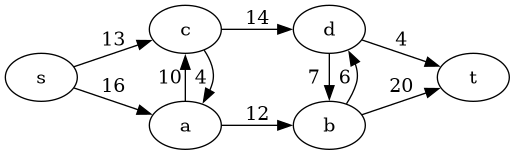
\includegraphics[scale=.3]{graph-example}}
    \end{center}
    %% you could just include the graphics without worrying about the \pause's;
    %% just comment the above lines and uncomment the following ones:
    
    %\begin{center}
    %   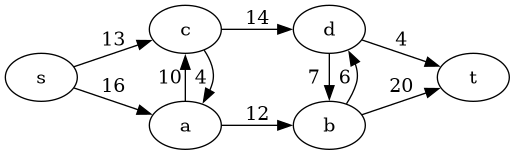
\includegraphics[scale=.3]{graph-example}}
    %\end{center}
  \end{itemize}
  
\end{frame}



\end{document}

